\section{Proposed System}\label{sec2a}

This section presents the comprehensive intelligent traffic light control network system that integrates Deep Reinforcement Learning (DRL) with computer vision technologies for adaptive traffic management. The proposed system employs a hierarchical architecture that combines local and global decision-making capabilities to achieve optimal traffic coordination across multiple intersections.

\subsection{System Architecture Overview}\label{subsec2a-1}

The proposed intelligent traffic light control system employs a three-layer hierarchical architecture designed to balance real-time responsiveness with network-wide optimization. Figure~\ref{fig:system_overview} illustrates the overall system architecture.

\begin{figure}[!htb]
    \centering
    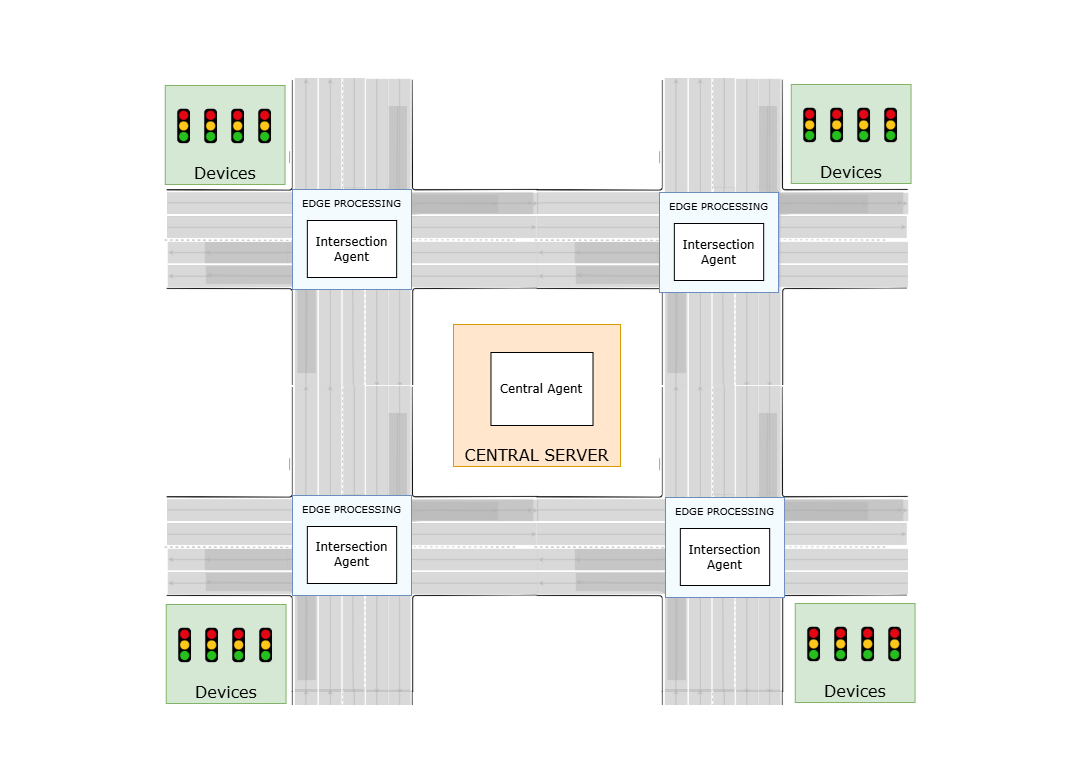
\includegraphics[width=0.8\textwidth]{figures/ch3_system_overview_architecture.png}
    \caption{Overall system architecture for intelligent traffic light control network}
    \label{fig:system_overview}
\end{figure}

The architecture consists of three main layers:

\textbf{Device Layer:} Surveillance cameras installed at traffic intersections capture real-time video streams of traffic conditions. These cameras are strategically positioned to provide comprehensive coverage of all approach lanes at each intersection, ensuring complete visibility of vehicle movements and traffic patterns.

\textbf{Edge Processing Layer:} Local computation devices at each intersection perform real-time vehicle detection, tracking, and local traffic signal control. This distributed approach minimizes communication latency and ensures immediate response to changing traffic conditions. Each intersection node operates independently while maintaining coordination capabilities with the central system.

\textbf{Central Server Layer:} A centralized coordination system collects information from all intersection agents, makes global optimization decisions, and provides a unified management interface for traffic operators. The central server implements the Sync Agent that coordinates multiple intersections for network-wide traffic flow optimization.

\subsection{Computer Vision Module}\label{subsec2a-2}

The computer vision module serves as the sensing component of the system, extracting comprehensive traffic information from camera feeds using state-of-the-art object detection and tracking algorithms.

\subsubsection{Vehicle Detection with YOLO11}

The system employs YOLO11s (You Only Look Once version 11 small), a pre-trained model that provides optimal balance between detection accuracy and processing speed for real-time traffic applications. YOLO11s achieves 47.0 mAP$^{50-95}$ on the COCO dataset while maintaining efficient processing speeds suitable for real-time traffic analysis on modern hardware.

YOLO11s offers several key advantages for traffic applications. The model provides balanced performance through high accuracy combined with fast inference speed suitable for real-time traffic monitoring. Its efficient architecture features enhanced backbone and neck designs with only 9.4 million parameters, ensuring computational efficiency. Additionally, the pre-trained capability enables direct application to traffic scenarios without additional training, with comprehensive support for vehicle classes including cars, motorcycles, buses, and trucks.

\subsubsection{Object Tracking Algorithms}

To maintain vehicle identities across video frames and extract trajectory information, the system implements two complementary tracking algorithms:

\textbf{SORT (Simple Online and Realtime Tracking):} Combines Kalman filters with Hungarian algorithm for efficient object tracking. The algorithm performs position prediction using motion models, object assignment based on IoU distances, and state updates with new detection information.

\textbf{BotSORT:} Enhances SORT by incorporating appearance-based features and improved motion models, providing superior tracking accuracy in complex scenarios with frequent occlusions and dense traffic conditions.

\subsection{Hierarchical Reinforcement Learning Architecture}\label{subsec2a-3}

The proposed system employs a two-level hierarchical DRL architecture that addresses both local optimization and global coordination challenges in multi-intersection traffic control.

\subsubsection{Local Level: DQN Agents}

Each intersection is controlled by a dedicated Deep Q-Network (DQN) agent responsible for local traffic signal decisions. The DQN architecture features an 80-dimensional input layer that captures comprehensive traffic state information by dividing each approach into 8 lane groups (2 groups per direction: straight/right-turn and left-turn lanes) with each group segmented into 10 spatial cells, creating an 8×10 = 80 element state vector. The network employs four fully connected hidden layers with 400 neurons each, utilizing ReLU activation functions for non-linear feature transformation. The output layer generates Q-values for four possible traffic phases: North-South green, East-West green, North-South left turn, and East-West left turn.

The action space is designed to cover standard four-way intersection control scenarios, while the state representation captures both spatial and temporal traffic dynamics necessary for intelligent decision-making.

\subsubsection{Global Level: SAC Agent}

The Sync Agent employs Soft Actor-Critic (SAC) algorithm to coordinate multiple intersection DQN agents. SAC is selected for its superior performance in continuous action spaces and its ability to maintain exploration-exploitation balance effectively.

The SAC agent observes aggregated information from all intersection DQN agents and makes comprehensive coordination decisions. These include phase duration adjustments for traffic wave coordination, priority assignments during emergency situations, load balancing across the intersection network, and synchronization timing optimization for enhanced traffic flow throughout the network.

\subsection{Reward Function Design}\label{subsec2a-4}

The reward functions are carefully designed to optimize multiple traffic objectives simultaneously while ensuring system stability and convergence.

For single intersection DQN agents, the local reward function is formulated as:
\begin{equation}
R_{\text{local}}(t) = W_{\text{total}}(t-1) - W_{\text{total}}(t)
\end{equation}

where $W_{\text{total}}(t)$ represents the cumulative waiting time of all vehicles at time step $t$. This difference-based approach directly rewards actions that reduce total waiting time, providing clear learning signals. When the action improves traffic flow, $W_{\text{total}}(t) < W_{\text{total}}(t-1)$, resulting in positive reward. Conversely, actions that worsen traffic conditions yield negative rewards.

For the global SAC agent, the reward function considers network-wide performance through a weighted combination approach:
\begin{equation}
R_{\text{global}} = 0.4 \cdot R_{\text{waiting}} + 0.3 \cdot R_{\text{queue}} + 0.3 \cdot R_{\text{speed}}
\end{equation}

where:
\begin{align}
R_{\text{waiting}} &= -\frac{\bar{W}}{100.0} \\
R_{\text{queue}} &= -\frac{\bar{Q}}{10.0} \\
R_{\text{speed}} &= \frac{\bar{V}}{50.0}
\end{align}

$\bar{W}$, $\bar{Q}$, and $\bar{V}$ represent the average waiting time, queue length, and vehicle speed across all intersections, respectively. The normalization factors ensure balanced contribution from each component.

\subsection{Training Methodology}\label{subsec2a-5}

The training process follows a three-stage approach to ensure stable learning and optimal coordination:

\textbf{Stage 1 - Individual DQN Training:} Each intersection DQN agent is trained independently using experience replay buffer with 100,000 transition capacity, target network updates every 1,000 steps, $\epsilon$-greedy exploration with decay from 1.0 to 0.1, and Adam optimizer with learning rate 0.001.

\textbf{Stage 2 - SAC Training with Fixed DQN:} The SAC agent learns coordination policies while keeping DQN agents fixed, using soft Q-learning with temperature parameter $\alpha = 0.2$, twin Q-networks to mitigate overestimation bias, and automatic entropy tuning for exploration-exploitation balance.

\textbf{Stage 3 - Joint Fine-tuning:} Both DQN and SAC agents are fine-tuned jointly with reduced learning rates to achieve optimal coordination while maintaining individual performance.

\subsection{Implementation Specifications}\label{subsec2a-6}

The system is implemented using modern software frameworks and hardware configurations optimized for real-time performance. TensorFlow 2.x serves as the primary deep learning framework for model development and deployment, while SUMO (Simulation of Urban Mobility) v1.22.0 provides the training and validation environment. Computer vision capabilities are enabled through Ultralytics YOLO11 integrated with OpenCV for real-time video processing. Agent coordination and data exchange utilize RESTful APIs as the communication protocol. Data management employs a hybrid approach with SQLite for local data storage and PostgreSQL for centralized data management. The hardware platform consists of Apple Mac Mini M2 with unified memory architecture, providing efficient model training and inference capabilities.

The system architecture supports real-time operation with efficient processing on modern unified memory architectures, ensuring responsive traffic control suitable for dynamic urban environments. The Apple M2 chip's neural engine acceleration provides optimal performance for both deep learning model training and computer vision tasks.
